\section{Week 2}
\subsection{Objective}
The objective of this week is to implement and experiment with Bayesian Optimal Design for Bayesian linear regression
as implemented in Week 1.
\subsection{Theory}
The Bayesian Optimal Design problem is about finding the a design $\B{d}$ from a design space $\B{D}$, that optimizes some kind of utility function.
For this project, that utility function is the mutual information gained from an experiment by measuring at "location" $\B{d}$.\\
Mutual information is in this case defined as
$$I(\B{d}) = \int_{\Theta}\int_{\B{Y}}p(\B{\theta}, \B{y}|\B{d})[\log p(\B{\theta}, \B{y}|\B{d}) - \log p(\B{y}|\B{d}) - \log p(\B{\theta})]d\B{y}d\B{\theta}$$
From last week, we assume that $p(\theta)$ (the prior in our linear model) is normally distributed with mean $\mu_\theta$ and covariance $\Sigma_\theta$.
We can condition $p(\B{\theta}, \B{y}|\B{d})$ on $\B{\theta}$ and get
$$p(\B{\theta}, \B{y}|\B{d}) = p(\B{\theta}|\B{y}, \B{d})p(\B{y}|\B{d})$$
such that 
% Here, $p(\B{\theta}|\B{y}, \B{d})$ is the posterior from last week, which we found also was normally distributed with
% $$\mu_{\B{\theta}| \B{y},\B{d}}=\Sigma_\theta \B{d}^T(\sigma_\B{y} I_N + \B{d}\Sigma_\theta \B{d}^T)^{-1} \B{y}$$
% $$\Sigma_{\B{\theta}| \B{y},\B{d}}=\Sigma_\theta  - \Sigma_\theta\B{d}^T(\sigma_\B{y} I_N + \B{d}\Sigma_\theta \B{d}^T)^{-1} \B{d}\Sigma_\theta$$
% We can then condition the joint distribution $p(\B{\theta}, \B{y}|\B{d})$ on $\B{y}$ and get
% $$p(\B{\theta}, \B{y}|\B{d}) = p(\B{y}|\B{\theta}, \B{d})p(\B{\theta}|\B{d})$$
% Since we know that the parameters of the underlying model are independent on the datapoints that are measured from, we have that $p(\B{\theta} | \B{d})=p(\B{\theta})$. 
% We also have that $p(\B{y}|\B{\theta}, \B{d})$ is the likelihood from last week, 
% which by assumption is normally distributed with mean $\theta^T\B{d}$ and covariance $\sigma_\B{y}^2$.
% Inserting our conditioning into $I(\B{d})$ gives us
% $$I(\B{d})= \int_{\Theta}\int_{\B{Y}}p(\B{y}| \B{\theta},\B{d})p(\theta)[\log p(\B{\theta}| \B{y}, \B{d}) - \log p(\B{\theta})]d\B{y}d\B{\theta}$$
\begin{align*}
  I(\B{d}) &= \int_{\Theta}\int_{\B{Y}}p(\B{\theta}, \B{y}|\B{d})[\log p(\B{\theta}| \B{y}, \B{d}) + \log p(\B{y}|\B{d}) - \log p(\B{y}|\B{d}) - \log p(\B{\theta})]d\B{y}d\B{\theta}\\
 &= \int_{\Theta}\int_{\B{Y}}p(\B{\theta}, \B{y}|\B{d})[\log p(\B{\theta}| \B{y}, \B{d}) - \log p(\B{\theta})]d\B{y}d\B{\theta}\\
 & \mbox{Split integral over $\B{Y}$}\\
 &= \int_{\Theta}\int_{\B{Y}}p(\B{\theta}, \B{y}|\B{d})\log p(\B{\theta}| \B{y}, \B{d}) d\B{y}- \int_{\B{Y}}p(\B{\theta}, \B{y}|\B{d})\log p(\B{\theta})d\B{y}d\B{\theta}\\
 & \mbox{Split joint distribution into conditional and marginal} \\
&= \int_{\Theta}\int_{\B{Y}}p(\B{\theta}, \B{y}|\B{d})\log p(\B{\theta}| \B{y}, \B{d}) d\B{y}- p(\theta)\log p(\B{\theta})\int_{\B{Y}}p(\B{y}|\B{\theta}, \B{d})d\B{y}d\B{\theta}\\
 & \mbox{Use that probability distributions integrate to 1} \\
&= \int_{\Theta}\int_{\B{Y}}p(\B{\theta}, \B{y}|\B{d})\log p(\B{\theta}| \B{y}, \B{d}) d\B{y}- p(\theta)\log p(\B{\theta})d\B{\theta}\\
  & \mbox{Split integral over $\Theta$} \\
&= \int_{\Theta}\int_{\B{Y}}p(\B{\theta}, \B{y}|\B{d})\log p(\B{\theta}| \B{y}, \B{d}) d\B{y}d\B{\theta}- \int_\Theta p(\theta)\log p(\B{\theta})d\B{\theta}\\
  & \mbox{Switch inner integral} \\
&= \int_{\B{Y}}\int_{\B{\Theta}}p(\B{\theta}, \B{y}|\B{d})\log p(\B{\theta}| \B{y}, \B{d}) d\B{\theta}d\B{y}- \int_\Theta p(\theta)\log p(\B{\theta})d\B{\theta}\\
 & \mbox{Split joint distribution into conditional and marginal} \\
&= \int_{\B{Y}}p(\B{y})\int_{\Theta}p(\B{\theta}|\B{y},\B{d})\log p(\B{\theta}| \B{y}, \B{d}) d\B{\theta}d\B{y}- \int_\Theta p(\theta)\log p(\B{\theta})d\B{\theta}\\
& \mbox{Use known integral of entropy (defined as $H(f) = \int_x f(x)\log f(x) dx$) }\\
& \mbox{for multivariate Gaussian distributions, as well as the fact that }\\
& \mbox{the prior and posterior are multivariate Gaussian.} \\
&= \int_{\B{Y}}p(\B{y})\frac{1}{2}\ln \det (2\pi e \Sigma_{\theta|\B{y,d}})d\B{y}- \frac{1}{2}\ln \det (2\pi e\Sigma_\theta)\\
& \mbox{Use that $\Sigma_{\theta | \B{y, d}}$ does not depend on $\B{y}$ (from last week)} \\
& \mbox{and that probability distributions integrate to 1} \\
&= \frac{1}{2}\ln \det (2\pi e \Sigma_{\theta|\B{y,d}})- \frac{1}{2}\ln \det (2\pi e\Sigma_\theta)\\
\end{align*}
To find the optimal design, we want to find a maximizer $\B{d}^*$ defined as such:
$$\B{d}^* = \arg \max_{\B{d}\in \B{D}} I(\B{d})$$
This can be done using an optimization approach, like a gradient-based line-search.
\subsection{Design}
The implementation is pretty straight-forward this week, as we only need to implement $I(\textbf{d})$ and plug it in to any out-of-the-box optimizer, such as \texttt{scipy.optimize.minimize(method="BFGS")}.\\
If one implements the optimization using \texttt{autograd.np}, the gradient can also be calculated easily, leading to a more efficient optimization approach.
\subsection{Results}
\begin{figure}
  \centering
  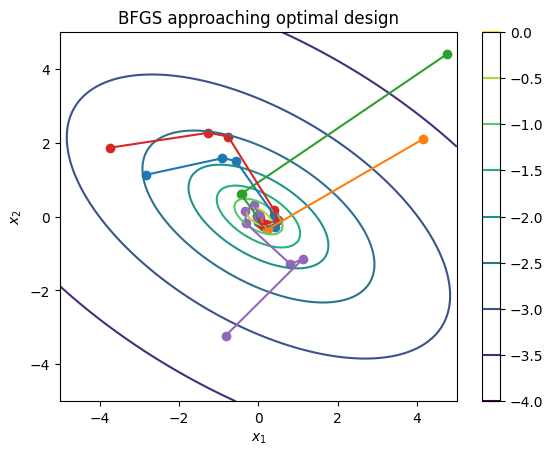
\includegraphics[width=0.8\textwidth]{week2/BFGS.png}
  \caption{BFGS algorithm optimizing for the most mutual information}
  \label{fig:BFGS}
\end{figure}
Running the BFGS algorithm 5 times with random start points over $I(\B{d})$ with $\Sigma_\theta=\begin{bmatrix}7.9 & 3 \\ 4 & 5\end{bmatrix}$ gives the plot seen in Figure \ref{fig:BFGS}. The algorithm usually converges after about 10 steps or so.
\subsection{Evaluation}
As it can be seen in Figure \ref{fig:BFGS}, the algorithm has no problem finding the optimal design for maximizing the mutual information between the prior and the posterior.
